
\tikzstyle{inputNode}=[draw,circle,minimum size=10pt,inner sep=0pt]
\tikzstyle{outputNode}=[draw,circle,minimum size=20pt,inner sep=0pt,red,thick,dashed]
\tikzstyle{stateTransition}=[-stealth, thick]

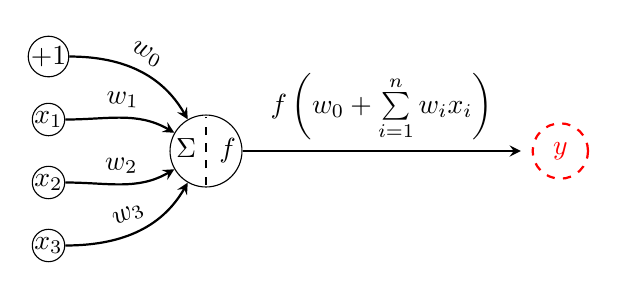
\begin{tikzpicture}
	
	\node[draw,circle,minimum size=26pt,inner sep=0pt] (x) at (0,0) {$\Sigma$ \, $f$};

	\node[inputNode] (x0) at (-2, 1.20)  {$\tiny +1$};
	\node[inputNode] (x1) at (-2, 0.40)  {$\tiny x_1$};
	\node[inputNode] (x2) at (-2,-0.40)  {$\tiny x_2$};
	\node[inputNode] (x3) at (-2,-1.20)  {$\tiny x_3$};

	\draw[stateTransition] (x0) to[out=0,in=120] node [midway, sloped, above] {$w_0$} (x);
	\draw[stateTransition] (x1) to[out=0,in=150] node [midway, sloped, above] {$w_1$} (x);
	\draw[stateTransition] (x2) to[out=0,in=210] node [midway, sloped, above] {$w_2$} (x);
	\draw[stateTransition] (x3) to[out=0,in=240] node [midway, sloped, above] {$w_3$} (x);
	
	\draw[stateTransition] (x) -- (4,0) node [midway,above] {$f\left(w_0 + \sum\limits_{i=1}^{n}{w_ix_i}\right)$};
	
	\node[outputNode] (y) at (4.5, 0) {$y$};
	
	\draw[dashed] (0,-0.43) -- (0,0.43);
	

\end{tikzpicture}